\documentclass[10pt,twocolumn,letterpaper]{article}
\usepackage[rebuttal]{cvpr}

% Preamble: packages
\usepackage{graphicx}
\usepackage{amsmath}
\usepackage{amssymb}
\usepackage{booktabs}
\usepackage[pagebackref,breaklinks,colorlinks,bookmarks=false]{hyperref}

% Document begins
\begin{document}

% Title and author
\title{Mini Project Report: CIFAR-10 Classification Under Data and Label Perturbations}
\author{김경환\\ Seoul National University}
\maketitle
\thispagestyle{empty}

% Abstract
\begin{abstract}
This report investigates the impact of altering data and label distributions on the performance of a simple convolutional neural network trained on CIFAR-10. We establish a baseline accuracy of 56.7% and compare it against three perturbation conditions: random label shuffle (6.1%), 20% label noise (50.5%), and strong input perturbation (47.4%). We present overall and per-class accuracies, confusion matrices, and training curves to illustrate how each manipulation affects model learning and generalization.
\end{abstract}

% Sections
\section{Introduction}
Image classification models often assume clean data and correct labels. However, in real-world scenarios, labels can be noisy and inputs perturbed. This study systematically analyzes how such imperfections degrade or sometimes improve model performance, using CIFAR-10 and a simple CNN implemented in PyTorch.

\section{Related Works}
Label noise has been shown to harm classification performance in various datasets~\cite{frenay2013classification,rolnick2017deep}. Data augmentation techniques, including random crops and blurring, can improve robustness~\cite{shorten2019survey}. Our work contrasts these effects directly under controlled perturbation fractions.

\section{Methods}
\subsection{Model Architecture}
We implement a two-layer convolutional network (SimpleCNN) with ReLU activations and max-pooling, followed by two fully connected layers. Training uses SGD with learning rate 0.01 and momentum 0.9.

\subsection{Perturbation Conditions}
Four experimental settings are defined:
\begin{itemize}
  \item \textbf{Baseline:} original CIFAR-10 labels and standard normalization.
  \item \textbf{Random Label Shuffle:} training labels fully permuted before each epoch.
  \item \textbf{Label Noise (20\%):} 20\% of training labels replaced randomly.
  \item \textbf{Input Perturbation:} random crops, horizontal flips, and Gaussian blur applied to inputs.
\end{itemize}

\subsection{Evaluation Metrics}
We report overall test accuracy, per-class accuracy, and confusion matrices. 

\section{Experiments}
\subsection{Setup}
All models trained for 10 epochs on a single GPU (or CPU) with batch size 128 for training and 100 for testing. Python and PyTorch implementations followed the unified script in \texttt{project.ipynb}.

\subsection{Results}
Table~\ref{tab:overall} summarizes overall accuracies. Figures~\ref{fig:overall_bar} and~\ref{fig:perclass_bar} visualize these results.

\begin{table}[t]
  \centering
  \begin{tabular}{l c}
    \toprule
    Condition            & Accuracy \\
    \midrule
    Baseline             & 56.7\%   \\
    Random Label Shuffle & 6.1\%    \\
    Label Noise (20\%)  & 50.5\%   \\
    Input Perturbation   & 47.4\%   \\
    \bottomrule
  \end{tabular}
  \caption{Overall test accuracy by condition.}
  \label{tab:overall}
\end{table}

\begin{figure}[t]
  \centering
  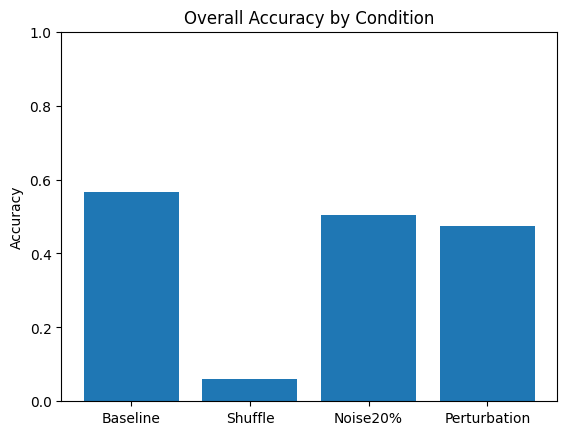
\includegraphics[width=0.8\linewidth]{overall_accuracy.png}
  \caption{Overall test accuracy across four conditions.}
  \label{fig:overall_bar}
\end{figure}

\begin{figure}[t]
  \centering
  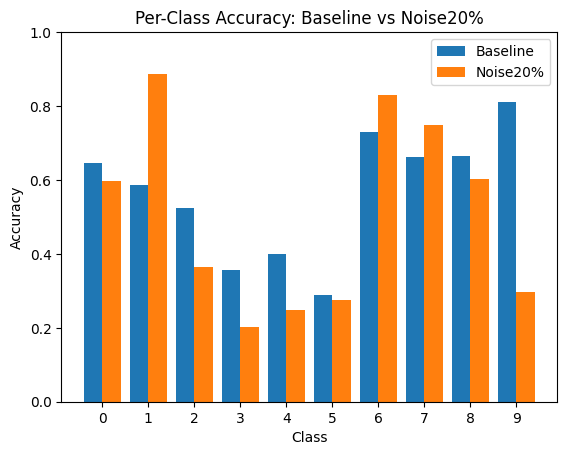
\includegraphics[width=0.8\linewidth]{per_class_accuracy.png}
  \caption{Per-class accuracy: Baseline vs. 20\% label noise.}
  \label{fig:perclass_bar}
\end{figure}

\section{Conclusion}
Our experiments confirm that label integrity is critical: random shuffle collapses performance to chance, while moderate noise degrades performance gracefully. Input perturbations (augmentation) yield robustness gains but do not reach baseline clean-label performance. Future work could explore higher noise fractions and advanced noise-robust training methods.

\begin{thebibliography}{9}
  \bibitem{frenay2013classification}
    F. Frenay and M. Verleysen,
    "Classification in the presence of label noise: a survey," 
    \textit{IEEE Trans. Neural Netw. Learn. Syst.}, vol. 25, no. 5, pp. 845--869, 2014.
  \bibitem{rolnick2017deep}
    D. Rolnick, A. Veit, S. Belongie, and N. Shavit,
    "Deep learning is robust to massive label noise," 
    \textit{arXiv preprint arXiv:1705.10694}, 2017.
  \bibitem{shorten2019survey}
    C. Shorten and T. M. Khoshgoftaar,
    "A survey on image data augmentation for deep learning," 
    \textit{Journal of Big Data}, vol. 6, no. 60, 2019.
    
\end{thebibliography}

\end{document}
